\documentclass{article}

% Based upon: https://tex.stackexchange.com/questions/32839/drawing-circuit-diagrams-with-logic-gates-in-latex
% https://tikz.dev/library-circuits

\usepackage{tikz}
\usetikzlibrary{arrows,shapes.gates.logic.US,shapes.gates.logic.IEC,calc}

\begin{document}

\thispagestyle{empty}
\tikzstyle{branch}=[fill,shape=circle,minimum size=3pt,inner sep=0pt]
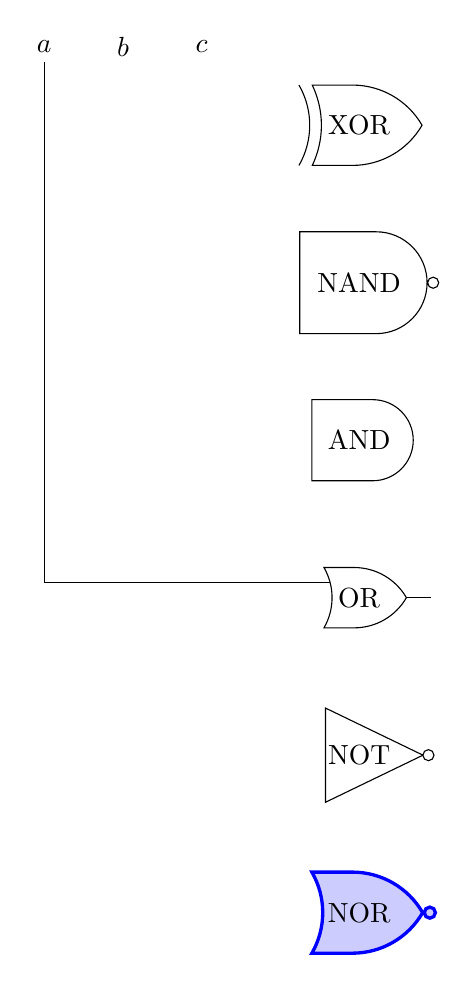
\begin{tikzpicture}[bluegate/.style={logic gate IEC symbol color=black,
    fill=blue!20,draw=blue,very thick}]
    
    \node (a) at (-3,7) {$a$};
    \node (b) at (-2,7) {$b$};
    \node (c) at (-1,7) {$c$};
    
    \node[nor gate US, draw, logic gate inputs=nnn, bluegate] at (1,-4) (GNOR) {NOR};
    \node[not gate US, draw, logic gate inputs=n] at (1,-2) (GNOT) {NOT};
    \node[or gate US, draw, logic gate inputs=nnn] at (1,0) (GOR) {OR};
    \node[and gate US, draw, logic gate inputs=nnn] at (1,2) (GAND) {AND};
    \node[nand gate US, draw, logic gate inputs=nnn] at (1,4) (GNAND) {NAND};
    \node[xor gate US, draw, logic gate inputs=nnn] at (1,6) (GXOR) {XOR};

    \draw (a.south) -- ++(south:0mm) |- (GOR.input 1);
    \draw (GOR.output) -- ++(right:3mm);
\end{tikzpicture}
\end{document}